\chapter{Introduction}\label{ch1}

The creation of a Style-Based Generator Architecture for Generative Adversarial Networks (StyleGAN) and similar technologies introduced the world to the possibility that images can be generated in such a way that it is difficult for a human to detect that these images are not real and instead generated by a neural network. With this proposed research project, the StyleGAN technology will be studied to determine how an approach can be developed to identify artificially generated images to enable the detection of these falsified identities that used the StyleGAN technology. An artefact will demonstrate the proposed solution methods function and convey the successful method in a practical environment with the use of StyleGAN generated images and images retrieved from the Flickr Faces dataset to evaluate the method. The following section is the proposal for the research project and will form the first chapter of this proposed project. In this Chapter, the background regarding the StyleGAN problem and a brief introduction to the StyleGAN technology will be explained. The Aims and Objectives will be set out to provide a clear goal and reference to the success of the final artefact. A Project management framework will be chosen and with the use of a Gantt chart will the timeline be structured to aid in the development of the artefact and completion of the project.

\section{Project Description}

StyleGAN is an open-source Generative Adversarial Network (GAN) that can be used to generate faces of people that do not exist (such as those shown on \href{https://www.thispersondoesnotexist.com}{thispersondoesnotexist.com}). This means that fraudsters can use StyleGAN generated faces that normally would pass a visual inspection conducted by a human inspector as part of false identities. The detection of such images with the use of artificial intelligence will be useful because of the factors that currently lead to misidentification.

\section{Project Background}

In this modern world with humanity currently in its 4th industrial revolution, the additions of innovative technologies require original approaches to implement and maintain these technologies. The change from the digital age to the automation age is accelerated by breakthroughs in the fields of Artificial Intelligence (AI) and security \citep{Skilton2017}.

One of the big advances in AI is the creation of StyleGAN, this new approach to a GAN allowed for more control in an image than its predecessors \citep{Karras2019}. StyleGAN uses the principles of a GAN to create new images derived from input that specifies what “styles” need to be included in the image. According to \cite{Karras2019}, a style is defined in this context as a set of parameters that modifies the input of the image to result in different outputs. If the input received is that the image needs to be in the style of a person with glasses, red hair and must be female, StyleGAN will then generate that image based on images used of that similar styles in the initial training of the model. The resulting image will thus be that of the “styles” required in the input. While this functionality can be utilized for various positive use cases – this breakthrough also creates various challenges and setbacks in the field of security, more specifically the aspects of facial recognition and identity verification as malicious use of this GAN might aid in the creation of fraudulent identities \citep{Mitra2021}. Figure \ref{fig:1} demonstrates how an image can be altered with the use of StyleGAN by specifying what style changes should be made on that image.

The styles applied in figure \ref{fig:1} demonstrate the capabilities of StyleGAN and further illustrate the possible difficulties of detecting that these images were generated with a GAN \citep{Karras2019}. Possible misidentification of StyleGAN images is a reality that needs to be addressed. Humans in the role of identifying artificially generated human faces may be susceptible to external factors hindering their capabilities and increasing the rate of error in which they identify fraudulent images \citep{Fysh2018}. \cite{Fysh2018} also noted that in the specific use case of passport officers that were tested on passport images captured on the same day against the “traveller” presenting that image, that the officers made substantial errors in a controlled environment when comparing the picture identity to that of the traveller. These results enforced their original statement that humans struggle with unfamiliar face identification.

Opportunities for fraud escalated with the recent boom in online applications. This bigger threat for fraud is exaggerated in the mobile market due to the high volume and demographic variety of current mobile users \citep{Mitra2021}. Most applications require user accounts and the unique user’s identity is commonly the specific value the application requires.

\begin{figure}[H]%
\centering
\fbox{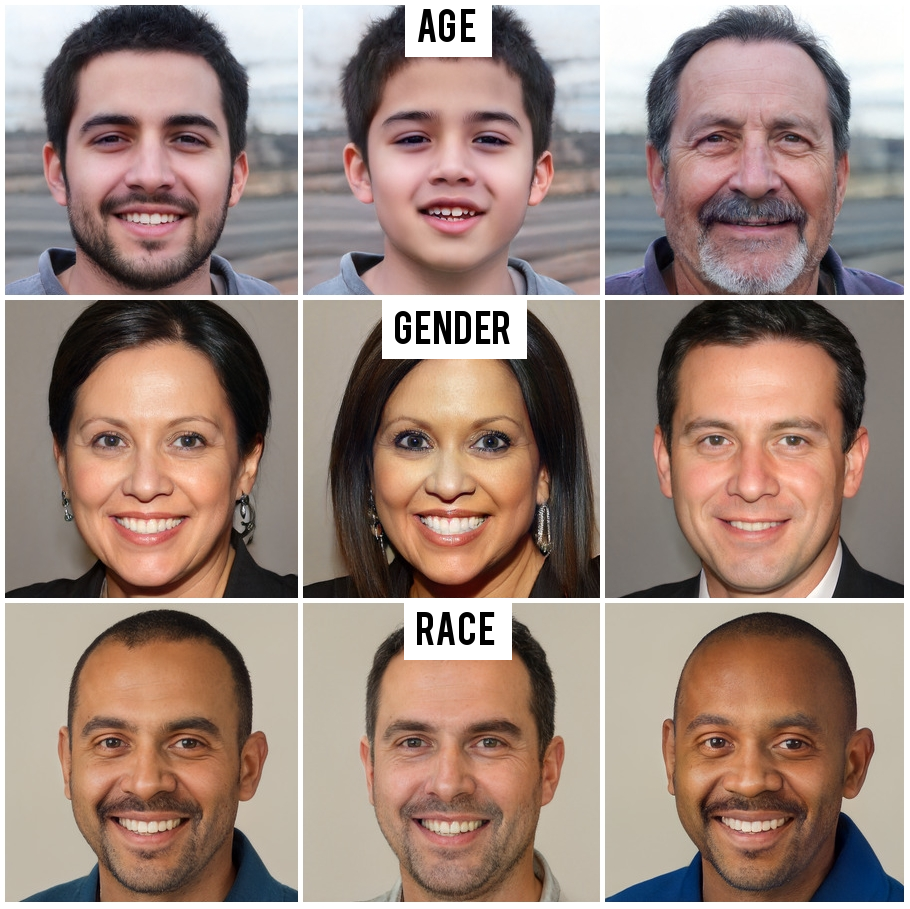
\includegraphics[width=0.95\textwidth]{img/f1.png}}%
\caption{Applied "styles" on images using StyleGAN that demonstrates styles and the resulting changes adapted from \cite{Karras2019}}%
\label{fig:1}%
\end{figure}

Examples of this in practice is online dating applications namely Bumble, Tinder and Hinge. These free to use applications allow multiple users to connect and interact where interaction mostly starts because of the user’s interaction with the images displayed on a profile. This emphasis on the gallery of a user profile creates a unique opportunity where StyleGAN can help cybercriminals fake identities within these apps. Fraudulent use of StyleGAN in this environment can directly lead to an increase in catfishing incidents. Catfishing is the act of deceiving an individual with the use of a specific fictional identity and persona to gain assets that are usually in the form of financial gains or personal information \citep{Chandler2016}. These apps usually have various systems in place to combat such fraudulent actions by requiring account verification. 

The verification process requests that a user submit one or multiple images where they pose in specific ways. StyleGAN can successfully counter these forms of verification as an image can be generated wherein a person perform specific poses \citep{Karras2019}. Example images of StyleGAN can be seen in Figure \ref{fig:sggg}. The diversity in StyleGAN images is another aspect of the GAN that ensures it can create very accurate images of humans that can go by undetected.

\begin{figure}[H]%
\centering
\fbox{\includegraphics[width=0.95\textwidth]{img/fsg.png}}%
\caption{Images from the StyleGAN dataset \cite{Karras2019}}%
\label{fig:sggg}%
\end{figure}

Because of StyleGAN’s ease of use and availability more fraudsters used it to create false accounts on popular social media platforms since its creation. Facebook took down an undisclosed number of accounts in December 2019 that had reportedly made use of StyleGAN to generate realistic profile pictures for establishing false identities on their site \citep{Gallagher2019}. This emphasized the possible threat StyleGAN poses to the security of individuals and the IT industry. Because of the threat, StyleGAN poses the need for a method to detect these generated images is identified. StyleGAN was released to the public in December 2018 with all its packages and source code. This novel approach to GAN’s that was developed by Nvidia demonstrated its possible capabilities by the accompanying portraits of convincing human faces. The big leap forward in this technology was the realism brought to the GAN’s generated faces dataset that is close to real human beings and not easily detected by humans \citep{Fleishman2019, Karras2019}.

StyleGAN was popularised because of a former engineer at Uber, Phillip Wang’s website \href{https://www.thispersondoesnotexist.com}{thispersondoesnotexist.com} that was released in February 2019. Phillip’s main goal when publishing this website was to educate the public on how GAN’s work and the dangers that they might pose to the average user. Phillip achieved this by specifically emphasizing StyleGAN and its realistic human face generation capabilities \cite{Fleishman2019}. The goal of making more people aware of StyleGAN and possible fake identities was also promoted by another website. Two members of the University of Washington created the website \href{https://www.whichfaceisreal.com}{whichfaceisreal.com} \cite{Fleishman2019}. This website allows users to select an image between a StyleGAN image and a verified human image. This online tool helped users realise that the differences between computer-generated images and real images are only decreasing with the advancement of technology.

The big advancement in StyleGAN that increased the need for this proposed project was the release of StyleGAN2 in February 2020 \citep{Karras2020}. Following the release of version 2, there were improvements in the generation process of these images with this updated version of StyleGAN. StyleGAN2 saw that images were no longer subverted with artefacts or traces left on the image because of the processing method used in the previous iterations \citep{Karras2020}. These traces were easy to identify and clearly showed out of place in the context of the image. With the removal of the traces, usually, in the form of drop-like spots, the difficulty in detecting the generated images increased and similarly the need to detect StyleGAN generated images used maliciously in security verification processes.

By looking at how the technology has been used since its release, the possible use-cases for GAN generated images and the always growing cybercrime industry the possible detection of these images is identified as a crucial function in the 4th industrial revolution. With these identified factors will the proposed project aim to solve the problem of detecting StyleGAN images by using an artificial intelligence approach to solve the problem.

\section{Research Question}

With the identified need for detection of StyleGAN images and the discussed security implications that the invention of StyleGAN and similar methods introduced the proposed project aims to detect these images with the use of a trained neural network. The main research question that this proposed project aims to answer is: How can StyleGAN generated images be detected?

\section{Aims and Objectives}
\subsection{Aims}

The main purpose of the proposed project is to develop a method that can detect fraudulent human faces created by StyleGAN with relative accuracy. Various techniques and approaches to the detection of GAN generated images will be researched and the simplest implemented approach that can still detect these types of images with relative surety will be selected for the artefact.

\subsection{Objectives}

The success of the project will be weighed against the completion of the secondary objectives that have been identified as listed below.

\begin{itemize}
	\item Perform a literature study on GAN's and specifically analyse the architecture and function of StyleGAN to understand the technology.
	\item Develop an approach to the successful identification of generated images.
	\item Develop an artefact that will use the selected method to detect a fake identity. 
\end{itemize}

The successful completion of the above-identified objectives will aid the researcher in satisfying the aim of the proposed research project. The success achieved in the creation of the method of detection will dtermine if the chosen method could consistenctly and in high frequency detected StyleGAN images in a pool of real and fake images. Only if the detection of the images is relatively high in the bounds of the project scope will the chosen method be implemented in the final artefact of this propsosed project.

\section{Procedures and Methods}

This section will describe the research paradigm and the methodologies that will be used to complete the proposed project. By examining the chosen paradigm, methodology and artefact life cycle in an academic viewpoint with specific reference to information systems design and development will the most applicable approaches in these sections be identified and selected. The data that will be captured in the development phase and reviewed in the testing phase will be discussed. Data capture in this proposed project will be the output metrics of the methods of detection performance and the retrieval of the datasets from their respective hosted repositories.

\subsection{Paradigm}

Positivism is a research paradigm that is focused on the world view that “factually accurate” knowledge is gained through the observations made by the observer. In positivistic studies, the research is confined to only the collection of data and the interpretation of this data to gain knowledge and insight into the problem. Positivism requires the researcher to only make quantifiable observations that can directly lead to statistical analysis. With the use of this paradigm, the researcher must reject intuitive knowledge because it cannot be justified by sensory experiences and is thus subjective to the researchers own interpersonal influences. Positivism as a philosophy is justifiable by empiricist views that knowledge stems from a human experience \citep{Collins2018}.

The positivistic research paradigm is suitable for the proposed project because with the creation of the artefact, the data collected will be examined and an unobjective interpretation of the data is necessary. The data collected will be the results of the artefact’s successful identification of StyleGAN generated images, and therefore a positivistic research paradigm will ensure the best method of detection is selected in the context of this proposed projects scope.

\subsection{Methodologies}

Methodologies determine the structure of completion for a specific project. With this proposed project the researcher will study the technology that enables StyleGAN to generate images. To aid in the research process and the development of the artefact the Design Science research methodology (DSRM) will be used throughout the proposed project \citep{Peffers2007}.

DSRM is an information systems specific methodology that focuses on research and iterative design \citep{Peffers2007}. Because the researcher is studying the field and technologies in which they want to solve the specific problem the background knowledge of the problem will be explored parallel to the design of the problem solution. DSRM will enable iterative design and development throughout the completion of the proposed project.

\subsection{Artefact Life Cycle}

With the use of the DSRM, the researcher will amend the project with the acquisition of new knowledge. The artefact will be developed while research is conducted on the technologies required, thus the artefact development will similarly be conducted in increments. The implementation of the Agile methodology for the development of the artefact will be suitable as Agile accommodates changes in artefact scope, planning and incremental deployments of preliminary artefacts \citep{Weiyin2011}.

The artefact that will be developed will aim to detect StyleGAN generated images between a data set of real images of human faces and StyleGAN generated images. The artefact can be hosted online if needed as this increase its compatibility and deployment reach across multiple platforms. Because of these factors, Agile will be the most suitable methodology for artefact development. 

\subsection{Data Capture}

The data captured in this project will be collected and displayed to the user in the web application to aid in the demonstration of the artefact, and method of detections success in the finalization phase of the project. Data that will be captured is the number of images used in the training of the models, the number of images that were used throughout the identification testing phase and the accuracy of the chosen identification method. These statistics will help the researcher determine the success of the chosen method of detection.

\section{Project Management and Project Plan}

\subsection{Scope}
The research of the technologies implemented in StyleGAN and the specific architecture of StyleGAN is important for the design of a suitable approach for the detection of these images. The scope of this research is the identification of images, the use of artificially generated human faces, security concerns when determining identities based on profile images and the research of neural network's that will be a possible technology used for the solution to the problem.

Because of the time of StyleGAN3 and 2 individual releases and the initialization of the proposed project the scope of this project will only focus on the detection of StyleGAN1 generated images. 


\subsection{Limitations}

Possible limitations that can be faced during the proposed project will hold back advancements that the researcher aims to complete in this study. The limitations thus need to be identified and addressed to ensure the completion of the proposed project within the specified period. The proposed project will make use of neural network's and image processing technologies to answer the research question. These technologies require large computing capabilities for the training of neural network models. This will be addressed by using cloud services instead of traditional hardware. Cloud services provide a more cost-effective approach to large computing needs.

\subsection{Risks}

Possible risks that can be identified that this proposed project is susceptible to include the risk that the scope of the project is not adhered to. The scope defines the boundaries in which this proposed project will take place, therefore careful adherence to the scope will ensure that the research is relevant to the initial project that was proposed. The responsibility of staying within the scope of the project lies in the researcher proposing this project.

\subsection{Strengths, Weaknesses, Opportunities and Threats}

The Strengths, Weaknesses, Opportunities and Threats (SWOT) of this proposed project can be evaluated using a SWOT-analysis table. The risks and limitations mentioned previously are also mentioned when conducting a SWOT analysis. Figure \ref{fig:2} shows the SWOT analysis of the proposed project.

\begin{figure}[H]%
\centering
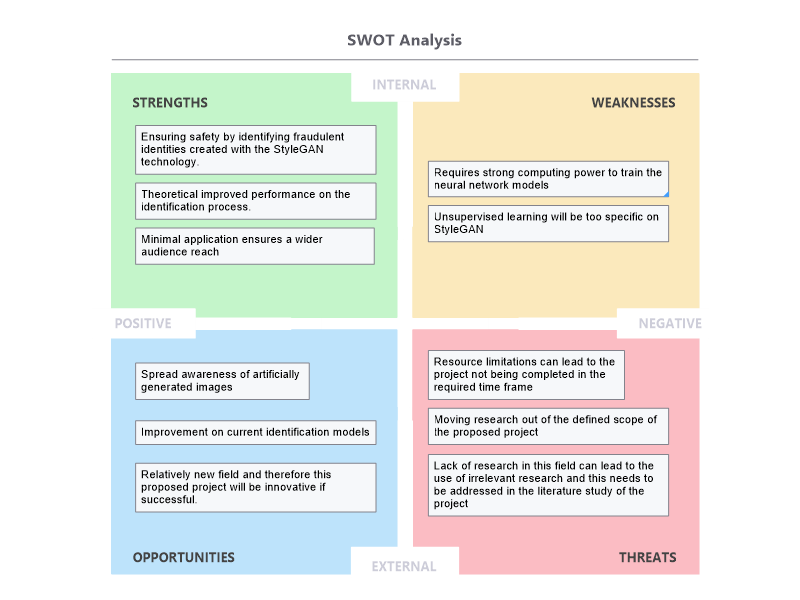
\includegraphics[width=1\textwidth]{img/SWOT.png}
\caption{SWOT analysis in the Identification of StyleGAN images}%
\label{fig:2}%
\end{figure}

\subsection{Timetable}

The proposed project will start on the 16\textsuperscript{th} of February 2021 and will be finalized and completed on the 8\textsuperscript{th} of November 2021. This project will be subdivided into 3 phases each with separate deadlines. The first phase is the research proposal that will be concluded on the 18\textsuperscript{th} of April 2021. The second phase involves research that will require an in-depth analysis of the problem, possible solutions, and the discussion of StyleGAN in a literature study that must be completed on the 13\textsuperscript{th} of June 2021. The last phase is the development of an artefact to practically demonstrate the solution to the identified problem. 

Phase 3 of the proposed project will also require a demonstration of the developed artefact and a video demonstration of the project on the 1\textsuperscript{st} of November 2021. The submission of the whole project must be completed and the final documentation will take place on the 8\textsuperscript{th} of November 2021. 

The Gantt chart in Figure \ref{fig:3} graphically displays the preliminary project planning with the tasks in the required sequential order for the successful completion of the proposed project. 

The adherence to the project planning and the preliminary Gantt chart will enable the researcher to effectively divide the tasks into manageable time frames. The prerequisite tasks are required to begin with a dependent task and are displayed graphically in figure \ref{fig:3}.

\begin{figure}[H]%
\centering
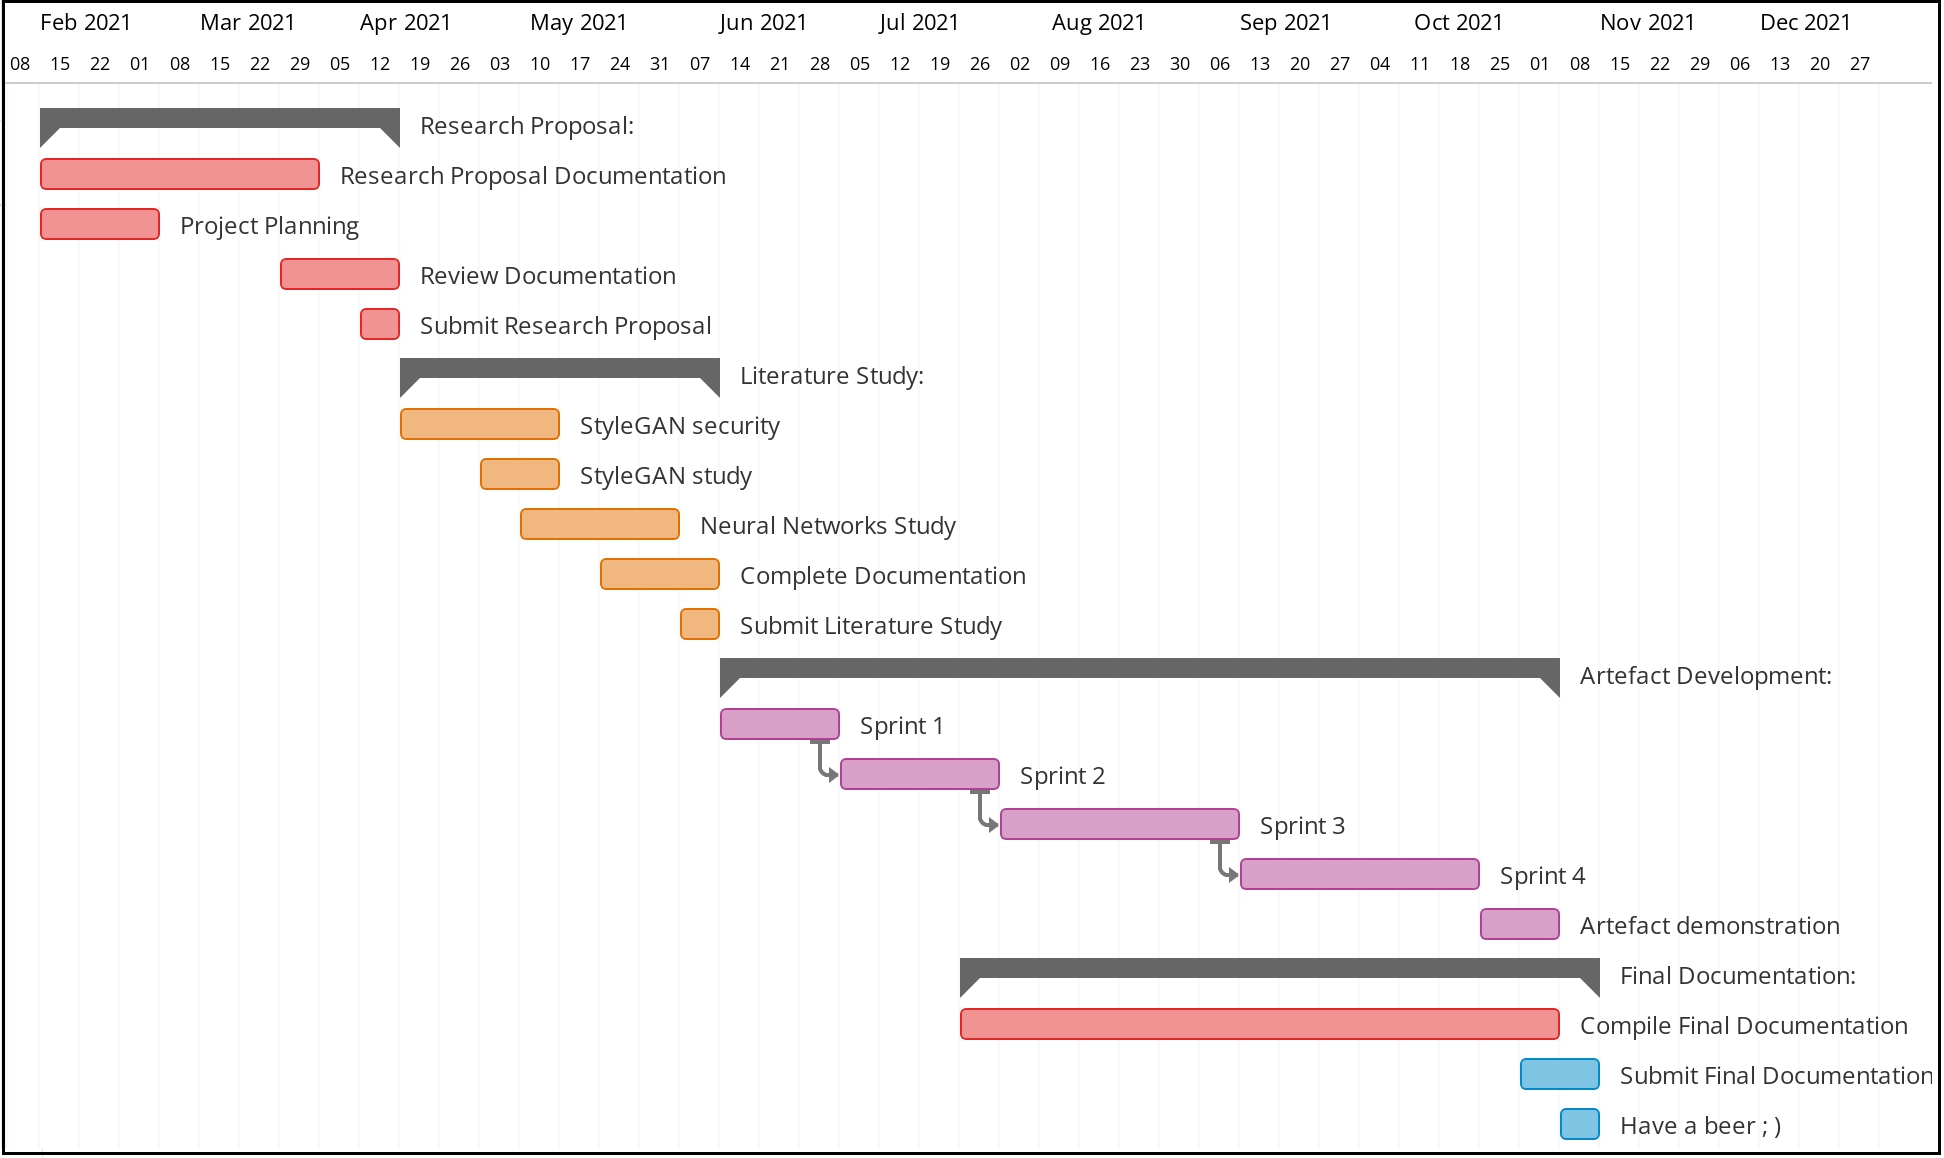
\includegraphics[width=1\textwidth]{img/ganttfinal.png}%
\caption{Gantt Chart graphically demonstrating the planned schedule of the proposed project}%
\label{fig:3}%
\end{figure}

In figure \ref{fig:3} time management and planning is clearly shown to be crucial for the completion of the proposed project. The artefact development planning is subject to change based on the research outcomes and findings of the researcher in this proposed project. 

\section{Development Platform, Resources and Environment}

The development of the artefact will be conducted in parallel with the research on the subject. Development of the GUI will be conducted at the same time as the literature study. The development of the final artefact and method of detection will only be conducted after the literature study based on the knowledge acquired in that phase. With the knowledge gained in the literature study will the specific method to detect StyleGAN images be implemented into the artefact. The artefact development platforms, resources and environments will be discussed in this section.

\subsection{Web Application}

The artefact will be a web application that can be scaled and hosted through a cloud services provider. The language that will be used for the front-end web application is Python-based using the scaled-down Django framework, Flask. For the implementation of the method for detection of StyleGAN generated images the language used in the back end of the artefact will be Python. The reasoning behind the selection of the above-mentioned technologies is discussed in the following section.

Developing a web-based application allows for further reach and compatibility compared to historical installation software \citep{murugesan2011}. Developing a simple web application with a minimalistic front end will users more intuitively be able to use the application and will improve complex implementations ease of use \citep{murugesan2011}. Web apps opened in the browser natively scale to be available on various devices and screen sizes. For the StyleGAN artefact, improved availability will provide the application with a wider reach and therefore more artificially generated images can be detected. 

The web application will allow a user to load a new image where the artefact will then classify that image as a StyleGAN generated image or a real human image. The web application must keep track of basic statistics and provide them to the user. The basic statistics that will be provided in the artefact of this proposed project will be the neural network's confidence in its prediction. An uncomplicated design will be implemented where the user can intuitively navigate the web page.

\subsection{Python}

For the backend of the proposed project Python will be used. Python is an intuitive programming language that due to its active community has an abundant set of resources available to use in the artificial intelligence field. Python is widely used for artificial intelligence applications and thus is a suitable programming language to code the chosen method of detection.

\subsection{Flask}

For the front-end of the artefact’s web application Flask will be used. Flask is a framework based on the larger framework Django that is a web framework using the Python language. Flask front-end features can use CSS-styling and the use of bootstrap will make the front-end uniform that enables faster development without the need for extensive visual design. Flask will enable the artefact to be used on multiple devices with a lightweight package without the explicit code and design to accommodate those devices. The framework natively scales assets to fit a wide range of devices.

\subsection{Jupyter Notebook}

Jupyter Notebooks is a Docker-like implementation of python coding. In a Jupyter notebook, cells can be run individually allowing for more control when developing neural network's. Most cloud services use Jupyter notebooks when implementing python code on their platforms. Jupyter notebooks are useful in data science and machine learning development because single python cell blocks can be executed. When training large neural networks that require long training times the cell blocks will prove useful because when training needs to be reinitiated for any reason the large code required beforehand does not have to be reinitiated.


\subsection{Cloud Services}

Because of the possible processing resource requirements that the detection of StyleGAN images require, the training of the neural network model will be conducted on the platform and infrastructure that is provided by Google Colab. A hybrid cloud services structure will be used in this proposed project because of the limited resources available.

\subsubsection{PaaS and IaaS}

In cloud services, there are multiple forms in which the cloud can be implemented for use by an individual or organisation. These implementations can range from Software to Infrastructure offered to the entity from the cloud services provider \citep{pfleeger2002}. For this proposed project there is a need for a platform and infrastructure as the training using large image datasets require processing power. Platform as a Service (PaaS) is a service model where the client develops software by using the languages and tools offered by the cloud services provider \citep{pfleeger2002}. Infrastructure as a Service (IaaS) is the second service model this proposed project will require. In IaaS the cloud services provider offers the use of processing resources and storage to name a few, to the client \citep{pfleeger2002}. A combination of IaaS and PaaS will be required for the completion of the artefact in this proposed project. 

\subsubsection{Google Colab with Drive}

Google Colab is a free service that Google offers to data scientists to use for the development of neural network's. Google Colab workbooks are the development platform in which programming is conducted that is similar to Jupyter Notebook development on local machines. The difference in using Google Colab is the increased system resources of the web-based virtual machine. Using Google Colab for the development in this project will have the benefit of the GPU attached development environment where a Nvidea K80 GPU with 12GB of RAM can be used. Google Drive is a storage solution offered by Google that is integrated with Google Colab. The large datasets can be uploaded to an NWU google accounts drive, where storage is unlimited. The dataset can be mounted in Google Colab using Google Drive.

\subsection{Git}

For version control and deployment, the Git language will be used and the repository for the development of the artefact will be hosted on GitHub. GitHub is integrated with various cloud services and this allows the developer to easily deploy and evaluate the code.

\subsection{Optuna}

The neural network hyperparameter optimization framework Optuna will be used to increase neural network performance  by optimizing the architecture of the network and the parameters within the network. Optuna is relatively new and will be studied while implementing the technology on the artefact using the DSRM.

\section{Ethical and Legal Implications}

With the development of this artefact, certain resources will be used to train the neural network. The training requires images that were generated by StyleGAN. For the comparison in the artefact images of real humans will be used. Figure \ref{fig:fliek} shows a sample of the real human images that will be used in this proposed project.

\begin{figure}[H]%
\centering
\fbox{\includegraphics[width=0.95\textwidth]{img/fflick.png}}%
\caption{Gantt Chart graphically demonstrating the planned schedule of the proposed project}%
\label{fig:fliek}%
\end{figure}

The StyleGAN generated images are available on the official StyleGAN GitHub repository. Included in this repository is trained StyleGAN models and multiple datasets of StyleGAN generated images. The licensing of these images is stated on the GitHub repository and is a Creative Commons license by NVIDIA Corporation \citep{Karras2019}. 

For the verified human faces, the preliminary dataset that will be used is the Flickr Faces dataset that was initially used to benchmark StyleGAN. The individual images were published in Flickr by their respective authors under either Creative Commons, Public Domain. All of these licenses allow free use, redistribution, and adaptation for non-commercial purposes \citep{Karras2019}.

\section{Provisional Chapter Division}

For this whole project, the following flow of the final document can be expected. These chapters will logically flow to aid in the understanding of the topic at hand and to ultimately ensure a successful artefact.

\subsubsection*{Chapter 1: Introduction}
This chapter will be concluded in the project proposal phase. It will include the research question, the project description and background. It will include the proposed project plan for the entire project.

\subsubsection*{Chapter 2: Literature Study}
This chapter will be comprised of all the necessary research to understand the project and fulfil the project aims and objectives. Mostly in this project will be focusing on the specific workings of StyleGAN to effectively detect fake images.

\begin{enumerate}
    \item StyleGAN: The history of StyleGAN and direct technologies that lead to this breakthrough in the field of GAN’s will be provided as well as the specific architecture of StyleGAN.
    \item Neural Network: This project will make use of Machine Learning and neural network's to detect StyleGAN generated images. A study will be completed on the field of artificial intelligence and how neural networks can aid in the detection of images.
    \item Hyperparameter Optimization will prove useful in improving the created neural network model to increase the detection accuracy for StyleGAN images. A Study on hyperparameter optimization methods will aid in the creation of a hyperparameter artefact.
\end{enumerate}

The study of these three sub-topics will provide the relevant background and base knowledge to develop a successful artefact and will provide the relevant foundation to improve and expand on this project in the future.

\subsubsection*{Chapter 3: Development of the artefact}

Chapter 3 will apply the chosen methodologies that were identified and discussed in Chapter 1 to enable the successful development of the proposed project's artefact. This chapter will document the artefact development phase including unfamiliar problems that are identified within the development stage. The success of the artefact will be compared to the Aims and Objectives of Chapter 1 and if they are met.

\subsubsection*{Chapter 4: Results}

The results of the Artefact will be introduced in this Chapter and the successful identification of StyleGAN images will be determined. The testing in this Chapter will identify the success of the artefact with the comparison in Chapter 4.

\subsubsection*{Chapter 5: Reflection}

Chapter 5 will summarize the entire proposed project and conclude if the problem was solved with the successful completion of the objectives of the proposed project that allowed it to fulfil the aim of the project. The limitations that impeded the proposed project will be discussed in this section. The future expansion of the project will be discussed and explained in the context of the limitations faced.

\section{Summary}

The creation of StyleGAN images has sprouted possible security issues where falsified images can be used to create false profiles on the internet. The detection of these images will prove useful in the growing cybercrime world. StyleGAN images can be detected by implementing a machine learning approach to the problem. This project will use the DSRM in combination with Agile to develop an artefact that will detect StyleGAN images. By analysing StyleGAN and NN in a literature review can the development of the artefact commence based on the findings in the literature study.


